\documentclass[12pt, a4paper]{article}
\usepackage[margin = 1in, top=1.3in]{geometry}
\usepackage[english]{babel}
\usepackage[utf8]{inputenc}
\usepackage{fancyhdr}
\usepackage[fleqn]{amsmath}
\usepackage{mathtools}
\usepackage{tabto}
\usepackage{bm}
\usepackage{graphicx}
\graphicspath{{./images/}}
\usepackage[font=small,labelfont=bf]{caption}
 
\pagestyle{fancy}
\fancyhf{}
\rhead{\small{Shaan Ul Haque(180070053)\\ Samarth Singh (180050090) \\ Niraj Mahajan (180050069)}}
\lhead{CS-663 Assignment-2 : Question 3}
\rfoot{Page 3.\thepage}
 
\begin{document}
\vspace*{-22pt}
\section*{Question 3}
\subsection*{3.1 Isotropic Gaussian Mask}
We used a gaussian mask of $\sigma$ = 1.5 to make the patches isotropic.
\renewcommand{\thefigure}{3.1}
\begin{figure}[h]
    \centering
    \vspace*{-15pt}
    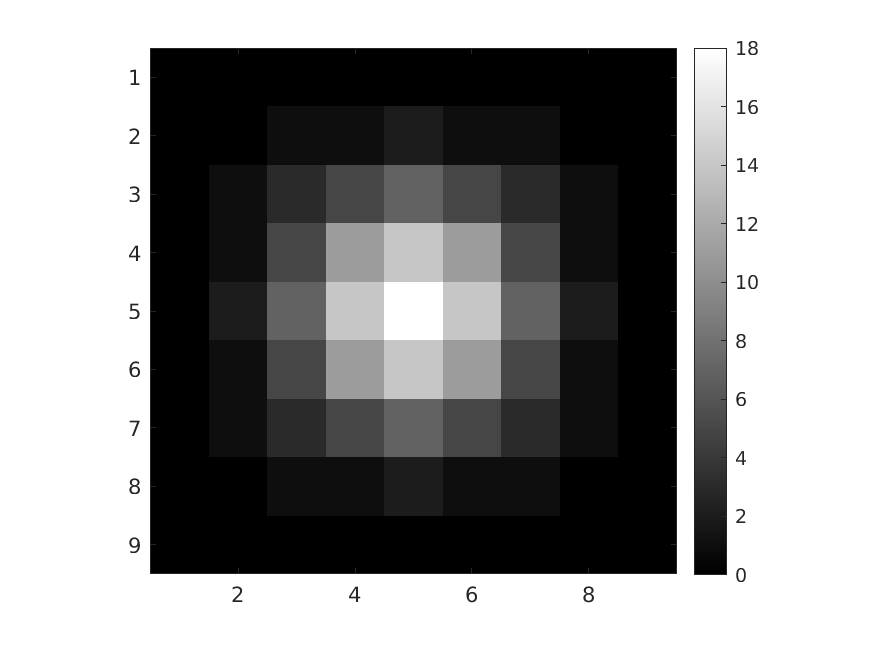
\includegraphics[width=0.5\textwidth]{isotropic_filter.png}
    \vspace*{-15pt}
    \caption{Gaussian Mask}
    \label{fig:2.6}
\end{figure}

\subsection*{3.2 Patch Based Filtering on barbara.png}
\noindent The optimal filtering for barbara.png was attained at $\sigma_{barbara} = 0.8424$. \\
The RMSD values are:
\begin{itemize}
	\item RMSD$_{\sigma}\;\;\;$  = 2.614193
	\item RMSD$_{0.9\sigma}$ = 2.636064
	\item RMSD$_{1.1\sigma}$ = 2.669242
\end{itemize}
\begin{figure}[h]
    \centering
    \renewcommand{\thefigure}{3.2(a)}
    \begin{minipage}[c][1\width]{0.3\textwidth}
    	\hspace*{-1in}
    	\includegraphics[width=1.5\textwidth]{barbara_original.png}
    	\caption{Original}
	    \label{fig:3.2(a)}
    \end{minipage}
    \renewcommand{\thefigure}{3.2(b)}
    \begin{minipage}[c][1\width]{0.3\textwidth}
    	\hspace*{-0.5in}
    	\includegraphics[width=1.5\textwidth]{barbara_corrupted.png}
    	\caption{Corrupted}
	    \label{fig:3.2(b)}
    \end{minipage}
    \renewcommand{\thefigure}{3.2(c)}
    \begin{minipage}[c][1\width]{0.3\textwidth}
    	\includegraphics[width=1.5\textwidth]{barbara_filtered.png}
    	\caption{Filtered}
	    \label{fig:3.2(c)}
    \end{minipage}
\end{figure}
\newpage
\subsection*{3.3 Patch Based Filtering on grass.png}
\noindent The optimal filtering for barbara.png was attained at $\sigma_{grass} = 1.8527$. \\
The RMSD values are:
\begin{itemize}
	\item RMSD$_{\sigma}\;\;\;$  = 7.336307
	\item RMSD$_{0.9\sigma}$ = 7.471906
	\item RMSD$_{1.1\sigma}$ = 7.474340
\end{itemize}
\begin{figure}[h]
    \centering
    \renewcommand{\thefigure}{3.3(a)}
    \begin{minipage}[c][1\width]{0.3\textwidth}
    	\hspace*{-1in}
    	\includegraphics[width=1.5\textwidth]{grass_original.png}
    	\caption{Original}
	    \label{fig:3.3(a)}
    \end{minipage}
    \renewcommand{\thefigure}{3.3(b)}
    \begin{minipage}[c][1\width]{0.3\textwidth}
    	\hspace*{-0.5in}
    	\includegraphics[width=1.5\textwidth]{grass_corrupted.png}
    	\caption{Corrupted}
	    \label{fig:3.3(b)}
    \end{minipage}
    \renewcommand{\thefigure}{3.3(c)}
    \begin{minipage}[c][1\width]{0.3\textwidth}
    	\includegraphics[width=1.5\textwidth]{grass_filtered.png}
    	\caption{Filtered}
	    \label{fig:3.3(c)}
    \end{minipage}
\end{figure}

\subsection*{3.4 Patch Based Filtering on beehive.png}
\noindent The optimal filtering for barbara.png was attained at $\sigma_{beehive} = 2.0842$. \\
The RMSD values are:
\begin{itemize}
	\item RMSD$_{\sigma}\;\;\;$  = 7.424229
	\item RMSD$_{0.9\sigma}$ = 7.545112
	\item RMSD$_{1.1\sigma}$ = 7.557518
\end{itemize}
\begin{figure}[h]
    \centering
    \renewcommand{\thefigure}{3.4(a)}
    \begin{minipage}[c][1\width]{0.3\textwidth}
    	\hspace*{-1in}
    	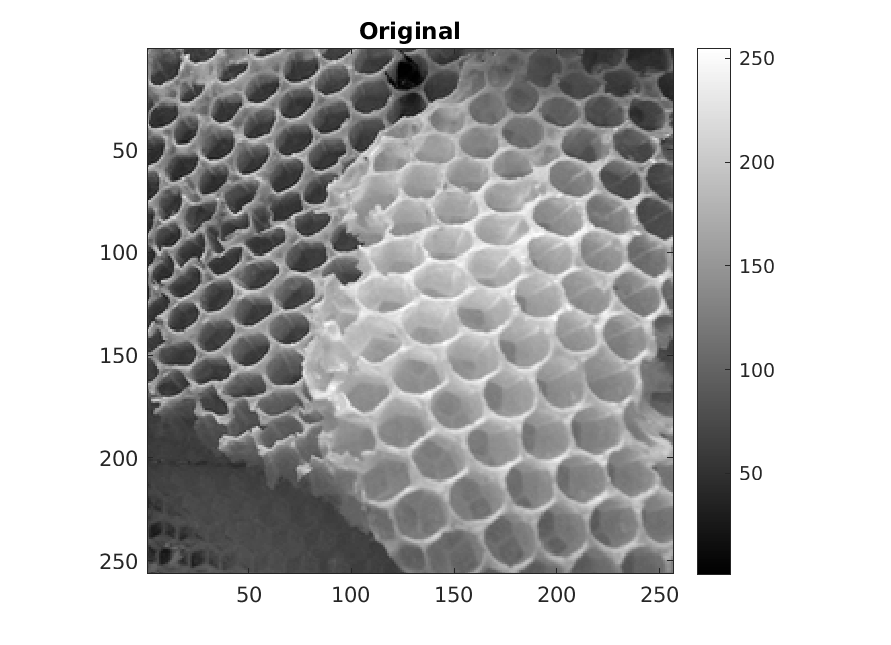
\includegraphics[width=1.5\textwidth]{Honeycomb_original.png}
    	\caption{Original}
	    \label{fig:3.4(a)}
    \end{minipage}
    \renewcommand{\thefigure}{3.4(b)}
    \begin{minipage}[c][1\width]{0.3\textwidth}
    	\hspace*{-0.5in}
    	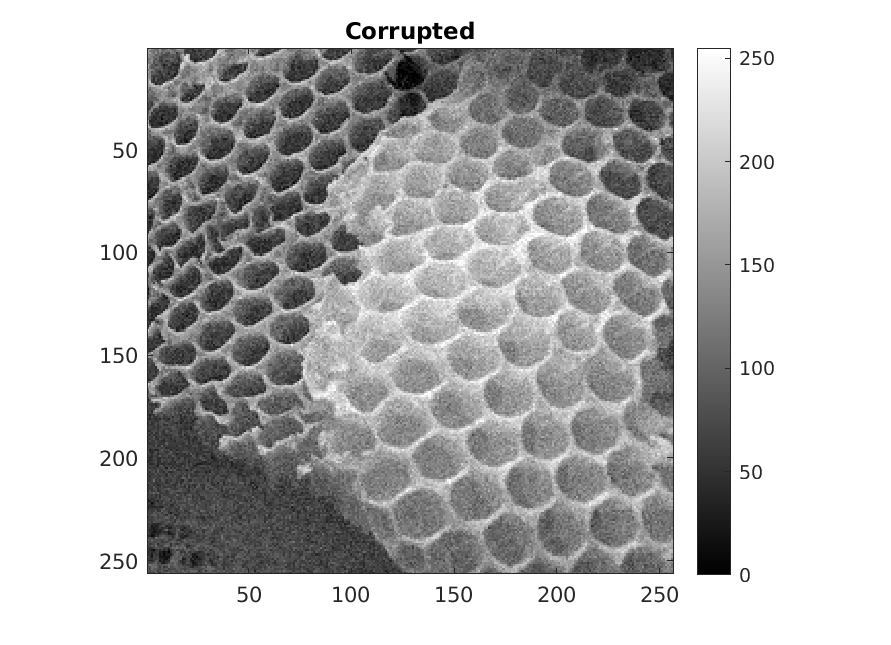
\includegraphics[width=1.5\textwidth]{Honeycomb_corrupted.png}
    	\caption{Corrupted}
	    \label{fig:3.4(b)}
    \end{minipage}
    \renewcommand{\thefigure}{3.4(c)}
    \begin{minipage}[c][1\width]{0.3\textwidth}
    	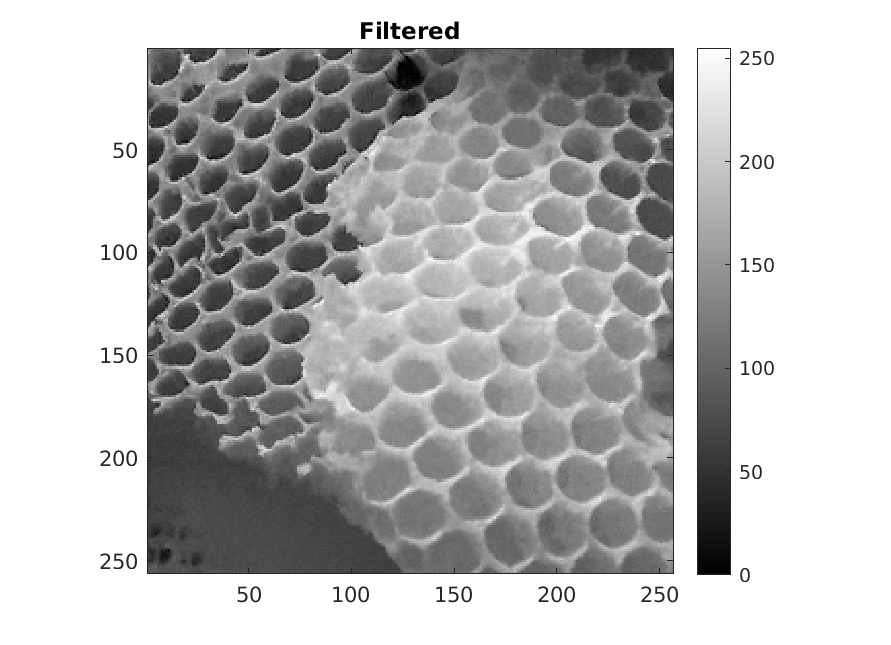
\includegraphics[width=1.5\textwidth]{Honeycomb_filtered.png}
    	\caption{Filtered}
	    \label{fig:3.4(c)}
    \end{minipage}
\end{figure}
\newpage
\subsection*{3.4 Usage of code}
\begin{itemize}
\item Running the \textbf{myMainScript.m} file will plot the original, corrupted and filtered images for all three test cases. This takes less than 5 minutes and hence wait bar is not shown.
\item By default, the 0.9$\sigma$ and 1.1$\sigma$  RMSD values will not be printed. In order to print these values, uncomment line 33 to 38 in \textbf{workOnImage.m}. Note that this will take 3 times the time required to run just for the optimal values and will exceed 5 minutes.
\item I have not scaled each image to [0,1] but simply converted the original pixel values to double and applied patch based filtering. This method is equivalent to scaling the image to [0,1], applying patch based filtering, and then rescaling to plot it. The quality of the filtered image will be the same. Just the $\sigma$ values and RMSD values will be scaled appropriately.\\ TL;DR: The RMSD values obtained by us will appear higher in magnitude as compared to those who have scaled the image to [0,1] but on scaling, the RMSD values are in the same range [let's hope better :)], and the filtered image quality is also the same [again, let's hope better :)]
\end{itemize}

\end{document}